\section{Introduction and Related Work}

Cacophony is a system that provides computational assistance with 
obtaining data from sources or sensors that are on the internet, but not always
available or up to date.  While it is designed to address contextual data
sources, including sources of data that are human authored, it can be applied
more generally.

\subsection{Scenario}

Consider a community relief worker who is organizing a sandbagging team in
response to a recent storm.  He lives in a river valley which is prone to
flooding and which contains a series of water level indicators which reports the
river's water level every four hours through Twitter~\cite{Starbird2010,flood}.
One particular stretch of the river threatens to cause a great deal of damage if it
overflows its banks, but the sensor associated with that stretch of the river is not
responding.

Fortunately this Twitter feed is paired with a \Cacophony node and when the
community relief worker queries the \Cacophony node, it responds with several
alternative views of the data.  The first is the last known value of the sensor
with a timestamp, the second is a predicted value for the sensor based on
current weather and nearby flood sensors and the third is a response from
another community relief worker that is near that stretch of the river.  From
this rich data set, the relief worker decides that a better use of his team would be 
to work at a different location for the day.  In the meantime he calls the local
relief worker to fix that sensor.

Later in the day, when he queries the sensor's \Cacophony node he sees that it
has been fixed, has been reporting levels that are rising and within predicted
ranges, but not yet threatening to flood.


\subsection{Privacy}

Unlike the Confab~\cite{Hong2004} system that is primarily concerned with
privacy management, \Cacophony offers only simplistic control for controlling
the presentation of data.  On the one hand because the basic configuration of \Cacophony
manipulates data that is publically accessible, it does not inherently introduce
new privacy risks.  Futhermore, a \Cacophony node does not necessarily monitor
data that is personal at all (e.g., the flood scenario).   However, if a
\Cacophony node \emph{is} paired with a source of data that is
personal, it becomes easier to see historic trends in that data which, if not
technically novel, creates new social concerns.  

Although \Cacophony is compatible with
the approach used in Confab, we implemented the widely supported robots protocol from the search
engine community~\cite{robotstxt}.  This enables publishers of data to restrict
a \Cacophony node from associating with data in the same way search engines
are restricted from indexing web pages.  This is a voluntary protocol that is
not enforced with technology (although it could be).

\subsection{Cloning}

\begin{figure}
	\begin{center}
		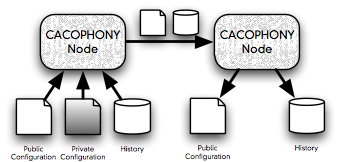
\includegraphics[width=1.00\columnwidth]{images/cloning}

	\caption{\label{fig:cloning}To clone a \Cacophony node the public
	configuration must be transferred.  Additionallly the historical data may be
	transferred.  The private configuration contains authentication credentials
	and is not transferred.}
	\end{center}
\end{figure}


A \Cacophony node is a java program that can be run on a standard java virtual
machine.  In order for the node to be valuable though, it needs to be connected
to the node that it is tracking and the nodes that are features for prediction.
Additionally it needs to observe those nodes over time to create a statistical
model of how they are correlated.  A node's state is therefore described by it's code,
it's connections and it's collected history.

In order to create a robust ecosystem of \Cacophony nodes, we support rapid
cloning of a node so that computation can be moved from one network location to
another.

The code of a \Cacophony node is open source and available online.  Since the
code is the same on all nodes, this aspect of it's state is easy to obtain.

The configuration of a \Cacophony node is separated into two files, a public
configuration file which contains information about which other nodes this node
connects to, and a private configuration file that contains access credentials
that may be required to instantiate those connections.  The public configuration
file can be obtained from any \Cacophony node via an http REST call.

The history of data that \Cacophony node has collected is contained in a local data store, initally
implemented as a SQLLite database.   This data is also available via a separate http
REST call.

In order to clone a \Cacophony node, one first downloads and executes the java
jar file from the \Cacophony website\footnote{What is the Cacophony website?} to
create the new node.
Then, via the web interface to the new node, the URL of the node to be cloned is
entered.  The new node requests the configuration of the old node and
reconfigures itself to match the network connections and data processing
parameters of the old node.  Once the configuration is complete, the history of
data collected is requested from the old node and stored in the new node's data
store.  Simply cloning the connections and bringing new \Cacophony node online takes less than a second under normal
network conditions.  Additionally transferring the history depends on the size
of the history and on current network conditions between the two nodes.






Cacophony consists of a set of computational nodes and data sources, distributed throughout the
internet, and connected in what is conceptually a directional graph.  Connections
represent communications that are passed between nodes via http/REST calls. Nodes are
aware only of themselves and the set of directly connected nodes.







Cacoph

If you consider sensors as delivering samples of the real world over time and
then send those samples through a network, the samples can be conceptualized as
a flow.to 


The idea of using data flows as perspective from which to manage contextual data
is heavily influenced by work in streaming databases and introduced to the
UbiComp community through the liquid system developed by Heer
et.al.~\cite{HeerNBH03}.  Liquid was a broad conceptual approach to context
aware data delivery that was inspired by work in streaming databases.  The
primary goal of liquid was to create links between nodes which incrementally
gathered, processed and delivered information to interested parties.

Cacophony is similar in that it also provides an architecture for connecting
computation nodes that deliver data from a source through a series of
transformations and aggregations to a sink node.

The main architectural difference between liquid and Cacophony is that liquid
made the assumption that the underlying data was continuously available.
Cacophony in contrast assumes that the underlying data is hidden and only
occassionally is an observation made that provides information about the hidden
variable of interest.  Cacophony assumes that the observations are noisy and not
always available.

Liquid also focussed on data discovery and alerting mechanisms.  Both of these
aspects of data aggregation are important, but are secondary to Cacophony's goal
of revealing hidden, occasionaly observable data.  Data discovery and alerting
mechanisms are both services that can be built on top of Cacophony and are not
central to it's focus on aggregation and statistical interpretation. 

Liquid and cacophony both take the perspective that context information is
maintained in a distributed fashion across multiple physical and organizational
boundaries.

Liquid makes some claims about it's ability to reroute queries in order to
follow mobile entities.  Cacophony does not attempt to reroute its data flows
beyond the mechanisms supported by the underlying networking protocols.  Once a
source of data is provided to Cacophony, Cacophony assumes that the data is
available at that location for all time.

In contrast, cacophony does provide robust mechanisms for rapid duplication of
streams.  

Another way of looking at cacophony is not as a competitor to liquid, but as a
wrapper for liquid. 

If liquid performs distributed "queries", Cacophony performs distributed
statistically learning of context.  Liquid's primary focus is data discovery,
cacophony is about robust prediction of context.

Cacophony is not really an architecture for "streaming data" as much as:
"streaming computation" which is presenting interpretations of instantaneous
data.

liquid encodes the idea of entities.  Cacophony supports entity prediction, but
doesn not expect a particular semantic on the underlying data.



Is there prior work before liquid?

What has come after liquid?  Does it relate?
\cite{Hong2004}



\subsection{Ideas}

The questions can be presented in a way that creates the least hassle for users
to answer i.e. Multiple Choice, Radio Button Ratings etc.

Their answers can be
stored and plotted on charts and graphs to give a flow of the general "time
based" information. 

For
example, a person wants get dinner at a restaurant, but doesn't want to be
bothered by long lines or noisy atmosphere. He can query Cacophony to find out
what the estimated wait time and atmosphere is like. 

Cacophony should also
present a percentage of accuracy based on the frequency of answered questions,
in a given time frame, for that location.



Example of pipe/ water flow and earthquake.
Swetak Patel

Respecting robots.txt


